\section{Examples}\label{sec:example}
This section will give three examples of our analysis of three different programs.
First, we provide a large example showing some possible program properties the analysis could answer and how it would be carried out.

After that, we provide the analysis of the program discussed in the introduction; as expected, the analysis terminates.
As it turns out, the cover lattices are superfluous in the first two examples.
More specifically if we let $\lookupcl(v) = \regexs_{\infty}$ or $\lookupcl(v) = \uints_{\infty}$ depending on the type of $v$, where $\regexs_{\infty}$ and $\uints_{\infty}$ is $\regexs$ and $\uints$ where transfinite union and intersection is allowed, respectively, the first two examples terminate.

For the sake of simplicity we assume the prequel in those respective examples.
Therefore, the last example is one where the cover lattice is needed.
In this example, we first show that the analysis does not terminate without the cover lattice and then show that it terminates with the cover lattice.


\subsection{Big Example}\label{subsec:big-example}
This section will present an example of a program that can be analyzed using the abstract interpretation presented in this paper.

The program in~\autoref{fig:program-code} is a simple program that simulates a bank system With delete, input, select, and update operations.
\begin{figure}
    \begin{minted}[frame=lines, linenos, escapeinside=||, mathescape=true]{text}
while true do(
    vName := [A-Z][a-z]* [A-Z][a-z]*;
    vBalance := |$\top$|;
    (Insert(account, <Name, Balance>, <vName, vBalance>), true)
)[](
    vName := |$\top$|;
    (delete(account), name = vName)
)[](
    vName := [A-Z][a-z]* [A-Z][a-z]*;
    toName := [A-Z][a-z]* [A-Z][a-z]*;
    amount := [0,+|$\infty$|];
    (select (vBalance, account, <name>), name = vName)
    (select (toBalance, account, <name>), name = toName)
    if(vBalance - amount) < 0
        then skip
    else(
        (update(account, <balance>, <vBalance - amount>), name = vName);
        (update(account, <balance>, <toBalance + amount>), name = toName);
    )
)
    \end{minted}
    \caption{Code for the program example}
    \label{fig:program-code}
\end{figure}

The program in~\autoref{fig:program-code} can be broken up into the following set of instructions, seen in~\autoref{eq:example-instructions-1} through~\autoref{eq:example-instructions-12}.

\begin{align} \label{eq:example-instructions-1}
    \begin{split}
    vName := [A-Z][a-z]* [A-Z][a-z]*;
    \end{split}
    & I_1\\
    \begin{split}
        vBalance := \top; 
    \end{split}
    & I_2\\
    \begin{split}
        &(Insert(account, <Name, Balance>, \\
        &<vName, vBalance>), true)
    \end{split} 
    & I_3\\
    \begin{split}
        vName := \top;
    \end{split} 
    & I_4\\
    \begin{split}
        (delete(account), name = vName)
    \end{split} 
    & I_5\\
    \begin{split}
        vName := [A-Z][a-z]* [A-Z][a-z]*;
    \end{split} 
    & I_6\\
    \begin{split}
        toName := [A-Z][a-z]* [A-Z][a-z]*;
    \end{split} 
    & I_7\\
    \begin{split}
        amount := [0,+ \infty];
    \end{split} 
    & I_8\\
    \begin{split}
        &(select (vBalance, account, <name>), \\
        &name = vName)
    \end{split} 
    & I_9\\
    \begin{split}
        &(select (toBalance, account, <name>), \\
        &name = toName)
    \end{split} 
    & I_{10}\\
    \begin{split}
        &(update(account, <balance>, \\
        &<vBalance - amount>), name = vName);
    \end{split} 
    & I_{11}\\
    \begin{split}
        \label{eq:example-instructions-12}
        &(update(account, <balance>, \\
        &<toBalance + vBalance>), name = toName);
    \end{split}
    & I_{12}
\end{align}

A program graph, seen in~\autoref{fig:full-graph-example} is then made from the program in~\autoref{fig:program-code} using the abstract interpretation.

\begin{figure}
    \centering
    \begin{tikzpicture}
    \tikzstyle{arrow} = [thick,->,>=stealth]
    \node [circle, draw] (start) at (0,0){$q_{\whitepointerright}$};

    \node [circle, draw] (a) at (0,-1) {};
    \node [circle, draw] (b) at (1,-1.8) {};

    \node [circle, draw] (c) at (-1,-1.8) {};
    \node [circle, draw] (d) at (-1,-2.8) {};
    \node [circle, draw] (e) at (-1,-3.8) {};

    \node [circle, draw] (f) at (-1,-4.8) {};
    \node [circle, draw] (g) at (-2,-4.8) {};

    \node [circle, draw] (h) at (2,-2.8) {};
    \node [circle, draw] (i) at (1,-3.8) {};
    \node [circle, draw] (j) at (2,-4.8) {};
    \node [circle, draw] (k) at (1,-5.8) {};
    \node [circle, draw] (l) at (2,-6.8) {};
    \node [circle, draw] (m) at (1,-7.8) {};

    \node [circle, draw] (n) at (2,-7.8) {};

    \node [circle, draw] (o) at (1,-8.8) {};
    \node [circle, draw] (p) at (3,-8.8) {};



    \node [circle, draw] (end) at (3,0) {$q_\blackpointerleft$};

    \draw[arrow, ->] (start) -- node[right]{true} (a);
    \draw[arrow, ->] (a) -- node[above, xshift=10, yshift=-4]{skip} (b);
    \draw[arrow, ->] (a) -- node[left, yshift=5, xshift=6]{skip} (c);
    \draw[arrow, ->] (c) -- node[right]{1} (d);
    \draw[arrow, ->] (d) -- node[right]{2} (e);

    \draw[arrow, ->] (b) -- node[right, yshift=-5, xshift=-4]{skip} (f);
    \draw[arrow, ->] (f) -- node[below]{4} (g);

    \draw[arrow, ->] (b) -- node[right, yshift=5, xshift=-4]{skip} (h);
    \draw[arrow, ->] (h) -- node[left, yshift=5, xshift=4]{6} (i);
    \draw[arrow, ->] (i) -- node[left, yshift=-5, xshift=3]{7} (j);
    \draw[arrow, ->] (j) -- node[left, yshift=5, xshift=4]{8} (k);
    \draw[arrow, ->] (k) -- node[left, yshift=-5, xshift=3]{9} (l);
    \draw[arrow, ->] (l) -- node[left, yshift=5, xshift=4]{10} (m);

    \draw[arrow, ->] (m) -- node[below]{B} (n);

    \draw[arrow, ->] (m) -- node[left]{$\neg$B} (o);
    \draw[arrow, ->] (o) -- node[above]{11} (p);

    \draw[arrow, ->] (start) -- node[above]{$\neg$true} (end);
    \draw[arrow, ->] (e) edge[bend left=45] node[left, yshift=-4]{3} (start);
    \draw[arrow, ->] (g) edge[bend left=50] node[left]{5} (start);
    \draw[arrow, ->] (n) edge[bend right=55] node[left]{skip} (start);
    \draw[arrow, ->] (p) edge[bend right=50] node[right]{12} (start);
\end{tikzpicture}
    \caption[short]{Full program graph example}
    \label{fig:full-graph-example}
\end{figure}


The program graph can then be simplified to the following program graph~\autoref{fig:simple-graph-example}.

\begin{figure}
    \centering
    \begin{tikzpicture}
\tikzstyle{arrow} = [thick,->,>=stealth]
    \node [circle, draw] (q0) at (0,0){$q_{\whitepointerright}$};
    \node [circle, draw] (qi) at (-2,0) {$q_i$};
    \node [circle, draw] (qd) at (2,0) {$q_d$};

    \node [circle, draw] (qt1) at (0,-2.7) {$q_{t1}$};
    \node [circle, draw] (qt2) at (0,-4.2) {$q_{t2}$};
    \node [circle, draw] (qt3) at (0,-5.7) {$q_{t3}$};
    \node [circle, draw] (qt4) at (-1.5,-6.5) {$q_{t4}$};
    \node [circle, draw] (qt5) at (1.5,-6.5) {$q_{t5}$};
    \node [circle, draw] (qt6) at (1.7,-8.4) {$q_{t6}$};
    \node [circle, draw] (end) at (-1.7,-8.4) {$q_\blackpointerleft$};

    \draw [arrow, ->](qd) edge[bend left] node[above]{$I_5$} (q0);
    \draw [arrow, ->](q0) edge[bend left] node[above]{$I_4$} (qd);
    \draw [arrow, ->](qi) edge[bend left] node[above]{$I_1;I_2$} (q0);
    \draw [arrow, ->](q0) edge[bend left] node[above]{$I_3$} (qi);

    \draw [arrow, ->](q0) -- node[right, yshift=-17]{$I_6;I_7;I_8$} (qt1);
    \draw [arrow, ->](qt1) -- node[right]{$I_9$} (qt2);
    \draw [arrow, ->](qt2) -- node[right]{$I_{10}$} (qt3);
    \draw [arrow, ->](qt3) -- node[left, xshift=2, yshift=5]{b} (qt4);
    \draw [arrow, ->](qt3) -- node[right, xshift=-5, yshift=5]{$\neg$b} (qt5);
    \draw [arrow, ->](qt5) -- node[left]{$I_{11}$} (qt6);

    \draw [arrow, ->](qt4) edge[bend left] node[right]{skip} (q0);
    \draw [arrow, ->](qt6) edge[bend right] node[right]{$I_{12}$} (q0);
\end{tikzpicture}
    \caption[short]{Simple program graph example}
    \label{fig:simple-graph-example}
\end{figure}

From the states of the program graph we get the following equations~\autoref{eq:example-equation-1} through~\autoref{eq:example-equation-12}.

\begin{align}
    \begin{split} \label{eq:example-equation-1}
        A(q_\whitepointerright)=A(q_\whitepointerright) &\cup \hat E_\whitepointerright \\&\cup \mathcal{\hat S} \lBrack skip \rBrack(A(q_{t4}))\\&\cup \mathcal{\hat S} \lBrack I_{12} \rBrack (A(q_{t6})) \\&\cup \mathcal{\hat S} \lBrack I_3 \rBrack (A(q_i)) \\&\cup \mathcal{\hat S} \lBrack I_5 \rBrack (A(q_d))
    \end{split}\\
    A(q_i)=A(q_i)&\cup \mathcal{\hat S} \lBrack I_1;I_2 \rBrack (A(q_\whitepointerright ))\\
    A(q_d)=A(q_d)&\cup \mathcal{\hat S} \lBrack I_4 \rBrack (A(q_\whitepointerright ))\\
    A(q_{t1})=A(q_{t1})&\cup \mathcal{\hat S} \lBrack I_6;I_7;I_8 \rBrack (A(q_\whitepointerright))\\
    A(q_{t2})=A(q_{t2})&\cup \mathcal{\hat S} \lBrack I_9 \rBrack (A(q_{t1}))\\
    A(q_{t3})=A(q_{t3})&\cup \mathcal{\hat S} \lBrack I_{10} \rBrack (A(q_{t2}))\\
    A(q_{t4})=A(q_{t4})&\cup \mathcal{\hat S} \lBrack b \rBrack (A(q_{t3}))\\
    A(q_{t5})=A(q_{t5})&\cup \mathcal{\hat S} \lBrack \neg b \rBrack (A(q_{t3}))\\
    A(q_{t6})=A(q_{t6})&\cup \mathcal{\hat S} \lBrack I_{11} \rBrack (A(q_{t5}))\\
    A(q_\blackpointerleft)=A(q_\blackpointerleft) \label{eq:example-equation-12}
\end{align}
    
When solving the equations seen in~\autoref{eq:example-equation-1} through ~\autoref{eq:example-equation-12} using the semantics in this paper, we get the following fixpoint~\autoref{eq:example-fixed-point-1} through~\autoref{eq:example-fixed-point-8}.

\begin{align}
    \label{eq:example-fixed-point-1}
    A(q_{\whitepointerright})=
    \begin{split}
        &\left\{\begin{matrix}
                   \left.\begin{matrix*}[l]
                             \texttt{vName}\\
                             \texttt{vBalance}\\
                             \texttt{toName}\\
                             \texttt{toBalance}\\
                             \texttt{amount}\\
                             \texttt{account}
                   \end{matrix*}\right|
                   \left.\begin{matrix}
                             \bot\\
                             \bot\\
                             \bot\\
                             \bot\\
                             \bot\\
                             \emptyset
                   \end{matrix}\right|
                   \left.\begin{matrix}
                             NR\\
                             \top\\
                             \bot\\
                             \bot\\
                             \bot\\
                             \mathsf{List} \; \{(NR,\top)\}
                   \end{matrix}\right|
                   \left.\begin{matrix}
                             \top\\
                             \bot\\
                             \bot\\
                             \bot\\
                             \bot\\
                             \emptyset
                   \end{matrix}\right|
        \end{matrix}\right.\\
        &\left.\begin{matrix}
                  \left.\begin{matrix}
                            NR\\
                            \mathsf{List} \; \{\top\}\\
                            NR\\
                            \mathsf{List} \; \{\top\}\\
                            +\\
                            \mathsf{List} \{(NR,\top)\}
                  \end{matrix}\right|
                  \left.\begin{matrix}
                            NR\\
                            \top\\
                            NR\\
                            \mathsf{List} \; \{\top\}\\
                            +\\
                            \mathsf{List} \{(NR,\top)\}
                  \end{matrix}\right|
                  \begin{matrix}
                      \top\\
                      \mathsf{List} \; \{\top\}\\
                      NR\\
                      \mathsf{List} \; \{\top\}\\
                      +\\
                      \mathsf{List} \; \{(NR,\top)\}
                  \end{matrix}
        \end{matrix}\right\}
    \end{split}
\end{align}

\begin{align}
    A(q_i)=\left\{\begin{matrix}
                      \left.\begin{matrix*}[l]
                                \texttt{vName}\\
                                \texttt{vBalance}\\
                                \texttt{toName}\\
                                \texttt{toBalance}\\
                                \texttt{amount}\\
                                \texttt{account}
                      \end{matrix*}\right|
                      \left.\begin{matrix}
                                NR\\
                                \top\\
                                \bot\\
                                \bot\\
                                \bot\\
                                \emptyset
                      \end{matrix}\right|
                      \left.\begin{matrix}
                                NR\\
                                \top\\
                                \bot\\
                                \bot\\
                                \bot\\
                                \mathsf{List} \; \{(NR,\top)\}
                      \end{matrix}\right|
                      \begin{matrix}
                          NR\\
                          \top\\
                          NR\\
                          \mathsf{List} \; \{\top\}\\
                          +\\
                          \mathsf{List} \; \{(NR,\top)\}
                      \end{matrix}
    \end{matrix}\right\}
\end{align}

\begin{align}
    A(q_d)=\left\{\begin{matrix}
                      \left.\begin{matrix}
                                \texttt{vName}\\
                                \texttt{vBalance}\\
                                \texttt{toName}\\
                                \texttt{toBalance}\\
                                \texttt{amount}\\
                                \texttt{account}
                      \end{matrix}\right|
                      \left.\begin{matrix}
                                \top\\
                                \bot\\
                                \bot\\
                                \bot\\
                                \bot\\
                                \emptyset
                      \end{matrix}\right|
                      \left.\begin{matrix}
                                \top\\
                                \top\\
                                \bot\\
                                \bot\\
                                \bot\\
                                \mathsf{List} \; \{(NR, \top)\}
                      \end{matrix}\right|
                      \begin{matrix}
                          \top\\
                          \mathsf{List} \; \{\top\}\\
                          NR\\
                          \mathsf{List} \; \{\top\}\\
                          +\\
                          \mathsf{List} \; \{(NR,\top)\}
                      \end{matrix}
    \end{matrix}\right.
\end{align}

\begin{align}
    A(q_{t_1})=
    \begin{split}
        &\left\{\begin{matrix}
                   \left.\begin{matrix*}[l]
                             \texttt{vName}\\
                             \texttt{vBalance}\\
                             \texttt{toName}\\
                             \texttt{toBalance}\\
                             \texttt{amount}\\
                             \texttt{account}
                   \end{matrix*}\right|
                   \left.\begin{matrix}
                             NR\\
                             \bot\\
                             NR\\
                             \bot\\
                             +\\
                             \emptyset
                   \end{matrix}\right|
                   \left.\begin{matrix}
                             NR\\
                             \top\\
                             NR\\
                             \bot\\
                             +\\
                             \mathsf{List} \; \{(NR, \top)\}
                   \end{matrix}\right|
        \end{matrix}\right. \\
        &\left.\begin{matrix}
                  \left.\begin{matrix}
                            NR\\
                            \mathsf{List} \; \{\top\}\\
                            NR\\
                            \mathsf{List} \; \{\top\}\\
                            +\\
                            \mathsf{List} \; \{(NR, \top)\}
                  \end{matrix}\right|
                  \begin{matrix}
                      NR\\
                      \top\\
                      NR\\
                      \mathsf{List} \; \{\top\}\\
                      +\\
                      \mathsf{List} \; \{(NR, \top)\}
                  \end{matrix}
        \end{matrix}\right\}
    \end{split}
\end{align}

\begin{align}
    A(q_{t_2})=\left\{\begin{matrix}
                          \left.\begin{matrix*}[l]
                                    \texttt{vName}\\
                                    \texttt{vBalance}\\
                                    \texttt{toName}\\
                                    \texttt{toBalance}\\
                                    \texttt{amount}\\
                                    \texttt{account}
                          \end{matrix*}\right|
                          \left.\begin{matrix}
                                    NR\\
                                    \emptyset\\
                                    NR\\
                                    \bot\\
                                    +\\
                                    \emptyset
                          \end{matrix}\right|
                          \left.\begin{matrix}
                                    NR\\
                                    \mathsf{List} \{\top\}\\
                                    NR\\
                                    \bot\\
                                    +\\
                                    \mathsf{List} \; \{(NR, \top)\}
                          \end{matrix}\right|
                          \begin{matrix}
                              NR\\
                              \mathsf{List} \{\top\}\\
                              NR\\
                              \mathsf{List} \{\top\}\\
                              +\\
                              \mathsf{List} \; \{(NR, \top)\}
                          \end{matrix}
    \end{matrix}\right\}
\end{align}

\begin{align}
    A(q_{t_3})=\left\{\begin{matrix}
                          \left.\begin{matrix*}[l]
                                    \texttt{vName}\\
                                    \texttt{vBalance}\\
                                    \texttt{toName}\\
                                    \texttt{toBalance}\\
                                    \texttt{amount}\\
                                    \texttt{account}
                          \end{matrix*}\right|
                          \left.\begin{matrix}
                                    NR\\
                                    \emptyset\\
                                    NR\\
                                    \emptyset\\
                                    +\\
                                    \emptyset
                          \end{matrix}\right|
                          \begin{matrix}
                              NR\\
                              \mathsf{List} \{\top\}\\
                              NR\\
                              \mathsf{List} \{\top\}\\
                              +\\
                              \mathsf{List} \; \{(NR, \top)\}
                          \end{matrix}
    \end{matrix}\right\}
\end{align}

\begin{align}
    A(q_{t_4})=\left\{\begin{matrix}
                          \left.\begin{matrix*}[l]
                                    \texttt{vName}\\
                                    \texttt{vBalance}\\
                                    \texttt{toName}\\
                                    \texttt{toBalance}\\
                                    \texttt{amount}\\
                                    \texttt{account}
                          \end{matrix*}\right|
                          \begin{matrix}
                              NR\\
                              \mathsf{List} \{\top\}\\
                              NR\\
                              \mathsf{List} \{\top\}\\
                              +\\
                              \mathsf{List} \; \{(NR, \top)\}
                          \end{matrix}
    \end{matrix}\right\}
\end{align}

\begin{align}
    \label{eq:example-fixed-point-7}
    A(q_{t_5})=\left\{\begin{matrix}
                          \left.\begin{matrix*}[l]
                                    \texttt{vName}\\
                                    \texttt{vBalance}\\
                                    \texttt{toName}\\
                                    \texttt{toBalance}\\
                                    \texttt{amount}\\
                                    \texttt{account}
                          \end{matrix*}\right|
                          \begin{matrix}
                              NR\\
                              \mathsf{List} \{\top\}\\
                              NR\\
                              \mathsf{List} \{\top\}\\
                              +\\
                              \mathsf{List} \; \{(NR, \top)\}
                          \end{matrix}
    \end{matrix}\right\}
\end{align}

\begin{align} 
\label{eq:example-fixed-point-8}
    A(q_{\blackpointerleft})=\emptyset
\end{align}


By using this, it is possible to analyze the program and check for some requested properties.
In this case one of the properties could be to check if it is possible to have accounts with a negative balance, which in this case would be possible.
Another case could be checking if it is possible to have accounts with names that are not in the format of the regular expression $[A-Z][a-z]^* [A-Z][a-z]^*$, which in this case would hold.

\subsection{Termination example}

\begin{figure}
    \centering
    \begin{tikzpicture}
    \tikzstyle{arrow} = [thick,->,>=stealth]
    \node [circle, draw] (start) at (0,0){$q_{\whitepointerright}$};
    \node [circle, draw] (a) at (0,-3) {$q_1$};
    \node [circle, draw] (end) at (0,-5) {$q_\blackpointerleft$};


    \draw[arrow, ->] (start) to node[left] {$true$} (a);
    \draw[arrow, ->] (a) edge[bend right=50] node[right]{($insert(...$} (start);

    \draw[arrow, ->] (start) edge[bend right=50] node[left]{$\neg true$} (end);
\end{tikzpicture}
    \caption{Termination example}
    \label{fig:termination-example}
\end{figure}

\subsection{Cover lattice example}


\begin{figure}
    \centering
    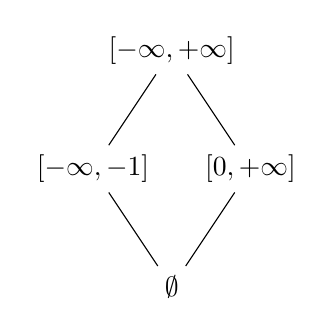
\begin{tikzpicture}
    \node (a)  at (0,0) {$[-\infty, +\infty]$};
    \node (b1) at (1,-1.5) {$[0,+\infty]$};
    \node (b2) at (-1,-1.5) {$[-\infty, -1]$};
    \node (c) at (0,-3) {$\emptyset$};
    \draw (a) to (b1);
    \draw (a) to (b2);
    \draw (b1) to (c);
    \draw (b2) to (c);
\end{tikzpicture}
    \caption{Termination example graph}
    \label{fig:termination-example-graph}
\end{figure}

\begin{figure}
    \centering
    \begin{tikzpicture}
    \tikzstyle{arrow} = [thick,->,>=stealth]
    \node [circle, draw] (start) at (0,0){$q_{\whitepointerright}$};
    \node [circle, draw] (a) at (0,-1.5) {$q_1$};
    \node [circle, draw] (b) at (0,-3.5) {$q_2$};
    \node [circle, draw] (end) at (0,-5) {$q_\blackpointerleft$};


    \draw[arrow, ->] (start) to node[right] {$i:=0$} (a);
    \draw[arrow, ->] (a) to node[left, xshift=2] {$true$} (b);

    \draw[arrow, ->] (b) edge[bend right=50] node[right]{$i:=i+1$} (a);

    \draw[arrow, ->] (a) edge[bend right=70] node[left]{$\neg true$} (end);
\end{tikzpicture}
    \caption{Cover lattice of the termination example graph}
    \label{fig:termination-example-cover-lattice}
\end{figure}
